\newpage
\section{Process Perspective}

%A description and illustration of:


%  - How do you interact as developers?
%  - How is the team organized?
%  - A complete description of stages and tools included in the CI/CD chains.
%    -  That is, including deployment and release of your systems.
%  - Organization of your repositor(ies).
%    - That is, either the structure of of mono-repository or organization of artifacts across repositories.
%    - In essence, it has to be be clear what is stored where and why.
%  - Applied branching strategy.
%  - Applied development process and tools supporting it
%    - For example, how did you use issues, Kanban boards, etc. to organize open tasks
%  - How do you monitor your systems and what precisely do you monitor?
%  - What do you log in your systems and how do you aggregate logs?
%  - Brief results of the security assessment.
%  - Applied strategy for scaling and load balancing.
%  - In case you have used AI-assistants for writing code during your project or to write the report:
%    - Explain which system(s) you used during the project.
%    - Reflect how it supported/hindered your process.


%In essence it has to be clear how code or other artifacts come from idea into the running system and everything that happens on the way.

\subsection{Teamwork}
\subsubsection{Team agreement}
Within the period where the project was worked, the team formed some rules and guidelines based on some of the points presented in the "Three Ways" to characterize DevOps from "The DevOps Handbook"\todo{Lets get a citation here}: Flow, Feedback and Continual Learning/Experimentation. This was to enhance efficiency, and to ensure transparency within the group.

\noindent To ensure flow we did the following:
\begin{itemize}
    \item Made work visible by using the GitHub kanban board.
    \item Reduced batch sizes by focusing on getting on feature done before moving focus to another.
    \item Reduced the number of handoffs by only working on a few features at a time,
    \item Continually identified and evaluated constraints by using GitHub issues if problems occurs.
    \item Eliminated hardship and waste in the value stream by implementing automatic releases in our pipeline.
\end{itemize}

\noindent To ensure feedback we did the following:
\begin{itemize}
    \item Discovered problems as they occur and make sure to communicate them to the team.
    \item Swarmed and solved problems to build new knowledge and share that knowledge with the rest of the group.
    \item Kept pushing quality closer to the source by using a trunk-based strategy that tested each push to the main branch.
\end{itemize}

\noindent To ensure continual learning and experimentation we did the following:
\begin{itemize}
    \item Institutionalized the improvement of daily work by keeping an open discussion about what we can do better.
    \item Injected resilience patterns into our daily work by using GitHub actions to constantly ensure quality of the work done.
    \item Ensuring a learning culture by by sharing knowledge at weekly meetings.
\end{itemize}

\subsubsection{Working schedule}
The team's interaction has been physical at ITU and online through Discord. The primary working day was Tuesday after the exercise session. The group would try to solve the exercise session first together, and then afterwards implement the feature to our own system. If there happened to be leftover work, we would split into subgroups, as different schedules made it difficult to meet physically more than once a week. Since most of the features and tools were new to the group the overall focus was to implement and use them in a correct manner. This led us to use pair programming, where one team member would share his screen and other team members provided input. In case the workload was trivial, the other team members would also write code individually. Furthermore, the team members who were not sharing their screen, would under many circumstances try to test or solve things on their own machines. This was to speed up the process, especially when we were working with something that we did not initially understand. \\

We incorporated retrospectives from Scrum every Tuesday before we began working on next weeks tasks. This meant that we discussed what had been implemented since last Tuesday as a way of sharing our individual knowledge with the group.

\subsection{CI/CD}
We used Github Actions to implement our CI/CD. Our CI/CD consists of test, deploy, release, and code quality analyzer. We used Trunk Based Development where every developer shared the same trunk branch. Every developer pushed to the main branch for efficiency. Upon push Github Actions will run the following steps:

\subsubsection{Code quality analyzer}
SonarCloud was used for code quality analyzer to analyze the technical debt of the code base. Our repository contains badges with information about the technical debt, security, vulnerabilities, and bugs based on the latest commit to SonarCloud. We also used the C\# linting tool \textit{code-cracker}, but this was only used when building on developer machines and not a part of the workflow. Furthermore, we have used Snyk for scanning the project, which er not a part of the workflow either.

\subsubsection{Test}
We have different tests as a quality gate before deploying and releasing. First, we have smoke test to verify that the most important elements of the application is functioning. Second, we use Selenium for end-to-end tests. Last, we use integration test in order to test the API.

\subsubsection{Deployment}
If the tests are successful the push will be deployed. We have omitted code reviews and branching in order to push new code faster. This is to prevent potential dead local code that is not being used, since we value that our code should be used, once it works.

\subsubsection{Release}
After deploying the application we use Versionize and Husky for automatic releases on Github.

\subsection{Repository organization}
We use a monorepository for our source code, both frontend and backend. As mentioned we have a trunk based development, which means that developers push directly to the main branch. If the commits passes the Github Workflow, then it will be released. We omitted code reviews because we thought it took too much time to do them, and since we often worked together physically, we mostly already knew what each other had written. Initially we considered using it for knowledge sharing, but since we were already set on using pair programming, we already had a way of knowledge sharing. Since we did not have code reviews we wanted to be able to release code as fast as possible.

\subsection{Development Process}
To track issues and which tasks needed to be done, we have to some degree utilized Github Projects, which provides Kanban boards. We have not used this feature rigorously, since the course structure already provided some structure of what needed to be done when. The main usage has been when we have split our group up in many parts (individual work), and needed to keep track of it. Mostly development has happened in group work, either all together or split in two groups with knowledge sharing. Since our project and group size are manageable, it is still possible to hold developers accountable by looking at commit history. A more rigorous use of the Kanban board would however have made it possible to retroactively measure system progress. 

\subsection{Monitoring \& Logging}
During the lifetime of a system, it is rare for everything to work smoothly and without any problems. System components will break down, the system will crash in production, server response times will grind to a halt, and so on. In order to (1) be able to estimate when the system is not operating within the expected limits, and (2) be able to track down the source of this disturbance, it is necessary to have monitoring and logging setup in the project.

Our monitoring is done via Grafana dashboards, where we have created two dashboards: One for system metrics (RAM, CPU usage, response times) and one for business logic (active users, timeline requests, number of tweets made). When the first dashboard showed irregular behaviour, it was a sign that our virtual machine in the cloud was in need of scaling - or that poorly performing code had been pushed recently. When the second dashboard showed irregular behaviour, it was a sign that our website was not deployed properly and inaccessible to users, or that some recently pushed code had broken core functionality.

In order to accurately track how many requests our system has in real time, we have implemented a logging tool. Each time a new user is created, an existing user logs in, a user makes a post, or a user follows another user, the API call is registered and saved in the logs. This gives us the ability to determine whether or not something is wrong, in case these API calls fail. 

\begin{figure}[H]
    \centering
    \subfloat[\centering A snippet of our logs showing the API calls registered]{{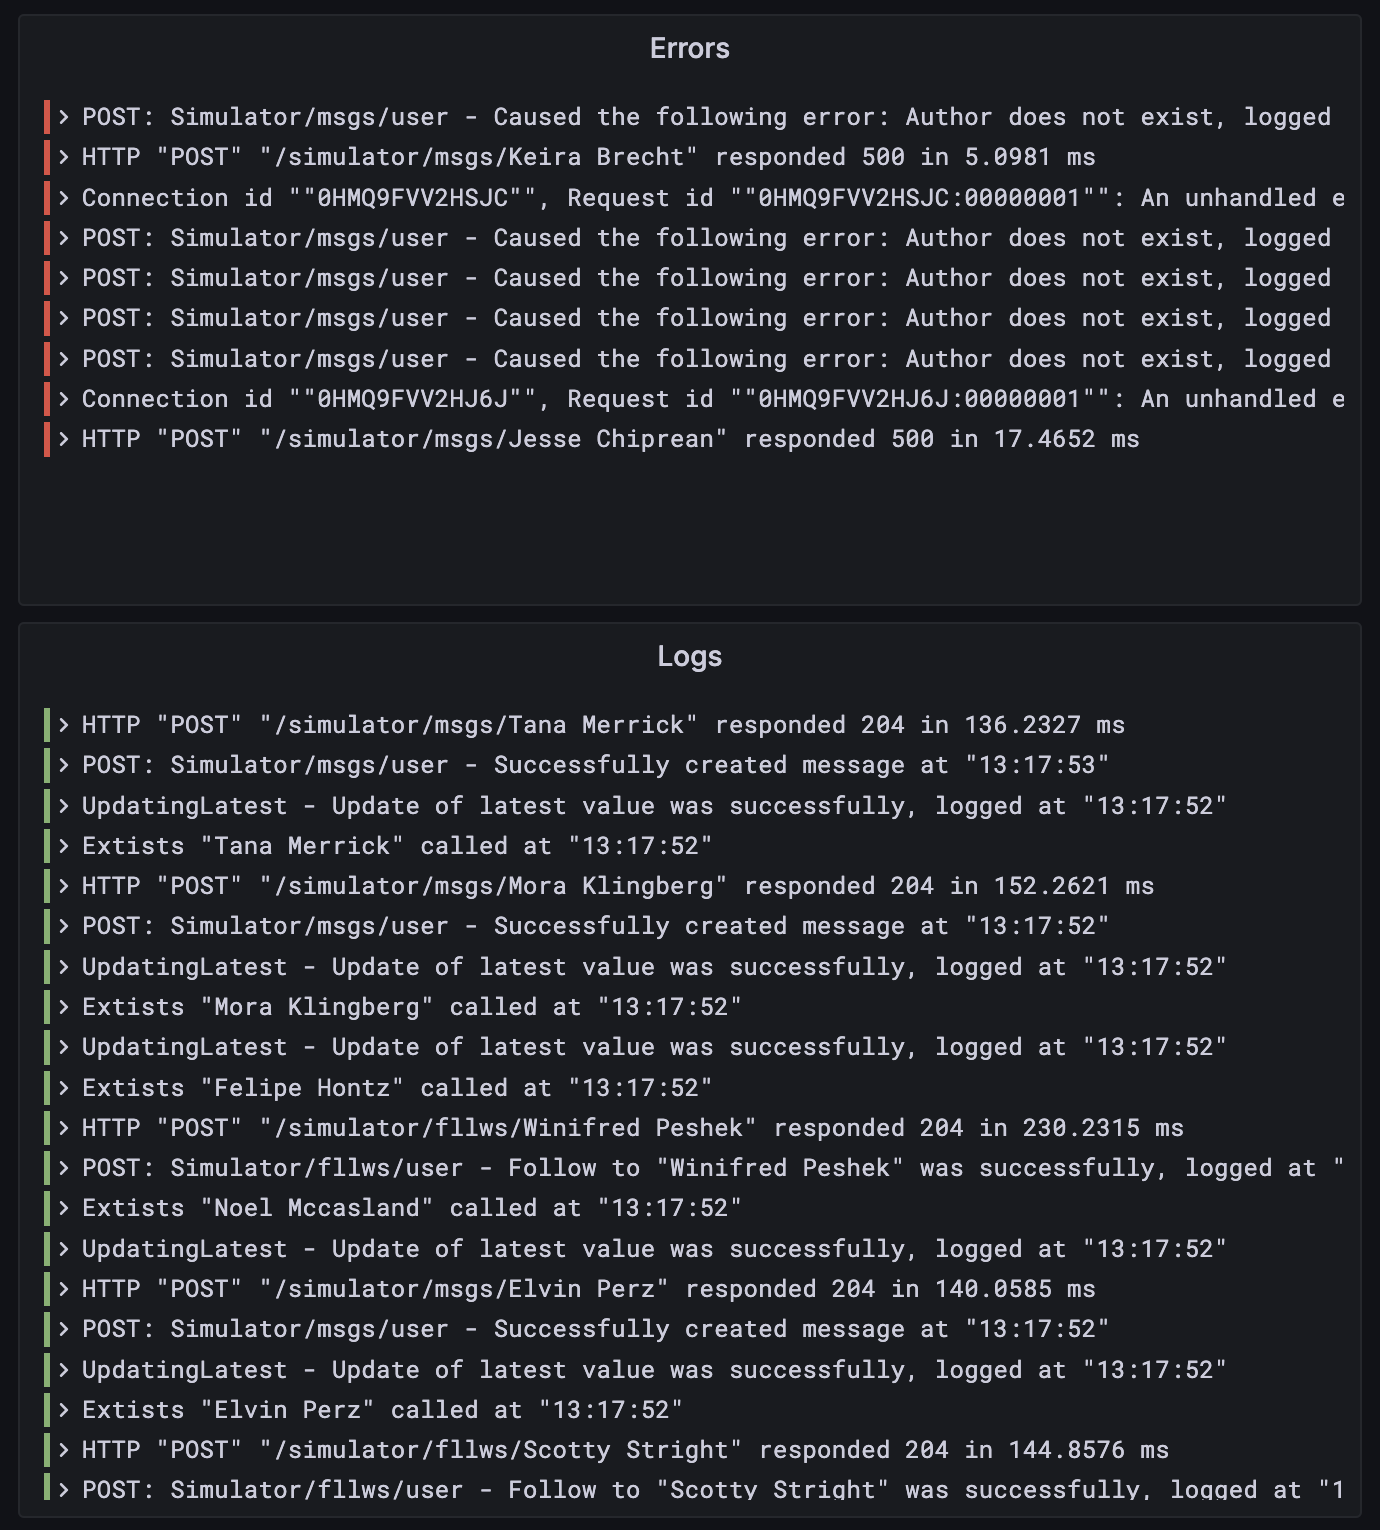
\includegraphics[width=0.45\textwidth]{images/logs_good.png} }}%
    \qquad
    \subfloat[\centering A snippet of our logs when we took down the database]{{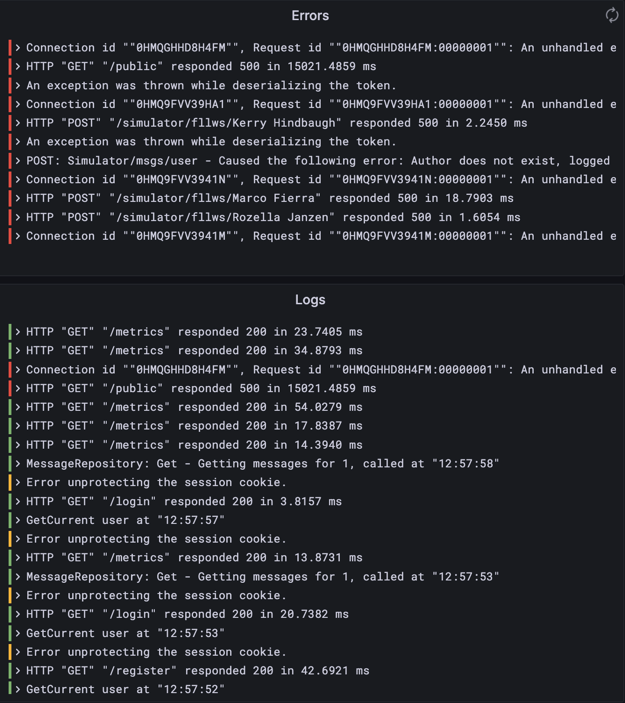
\includegraphics[width=0.45\textwidth]{images/logs_bad.png} }}%
    \caption{2 Figures side by side}%
    \label{fig:example}%
\end{figure}

When we had to change the database, we first had to take it down. This is visible in our logs, since we began getting a lot of errors when this was the case. This was ultimately a good sign, since it meant that if something was wrong in our system, we would be able to see it immediately, and therefore fix it as fast as possible.

\subsection{Scaling And Load Balancing}
Our load balancing is separated for a 'normal' user and the course simulator. When a request is made through the simulator API, we have decided to use a round robin approach to load balancing, which essentially means that the request is just sent to some container. However, when a connection is established through the website, we are using an IP hash approach. This means that the same user is always directed to the same container, which ensures that we do not have to worry about the user changing session states when the connection is renewed.

It has not been necessary to establish a scaling strategy, due to the scope of the course. Our monitoring has never indicated this to be necessary. If our current system would be overloaded, it would be necessary to either scale vertically or horizontally. Our system makes it easy to scale horizontally, the only real change being having to change our infrastructure as code scripts. Scaling vertically is easy through Digital Ocean.

\subsection{Security Assessment}
To discover potential security flaws in our system implementation, we decided to do a security assessment. This was done through the following process: 
\begin{enumerate}
    \item Identifying the different components of the system.
    \item Identify which component posed potential security breaches, and what these were for each component.
    \item Constructing risk scenarios on each potential security breach.
    \item Performing a risk analysis on the different scenarios.
    \item Running a preemptive pen-test on our own system.
\end{enumerate}

\begin{figure}[H]
    \centering
    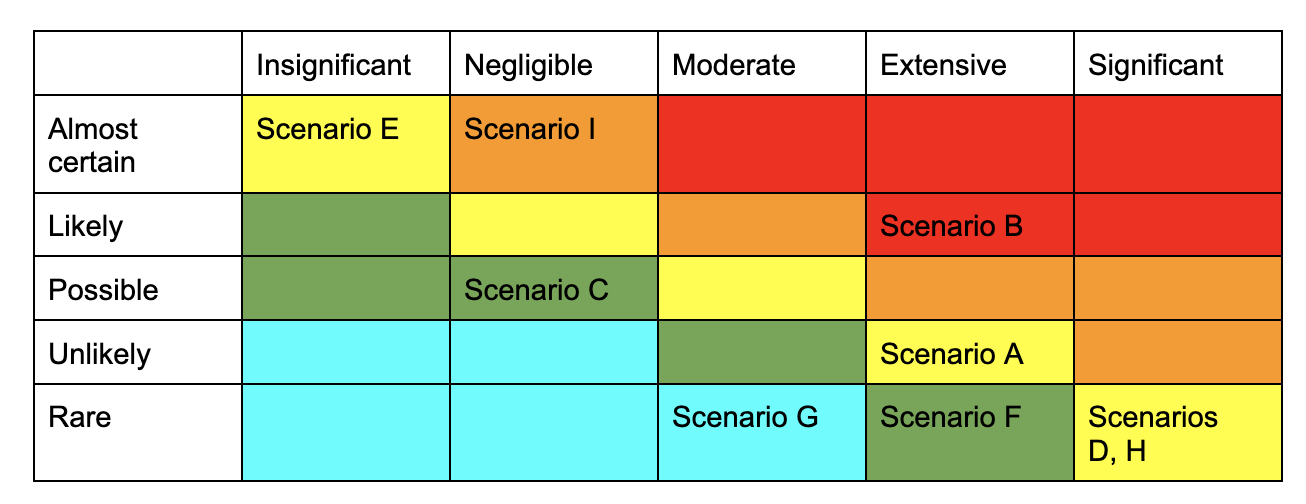
\includegraphics[width=0.8\textwidth]{images/securityAssessment.png}
    \caption{Security assessment of different risk scenarios (see appendix \ref{appendix:securityAssessment} for details on each scenario).}
    \label{fig:securityAssessmentTable}
\end{figure}

A report of our entire process can be found in appendix \ref{appendix:securityAssessment}. The security assessment, which this table stems from, can be seen in figure \ref{fig:securityAssessmentTable}. The table shows us that the most critical scenario is (B) Attacker performs a DDOS attack to make our server unresponsive. This would make our service useless, and could be very bad for the business. There is however no imminent way to mitigate this, other than scaling the application, having a load balancer, or pay for DDOS protection. Our system has a load balancer, but the other options were deemed to be outside the scope of this project.

While the security assessment has helped us realize which parts of the system is most vulnerable, and how they might be attacked, it does in no way guarantee that our system is unexploitable, or that every possible scenario is considered. The most normal way to discover security flaws is when an attacker takes advantage of them. The security assessment did however give us confidence that the most normal tools for discovering weaknesses didn't find anything on our system. Based on our findings, it was not necessary to change any parts of the system.

\subsection{AI assistants}
In this project we used ChatGPT. It did not write any of our source code, but it turned out to be helpful for error handling. When googling an error, it can sometimes be difficult to find the correct stack overflow response, whereas when using ChatGPT, we could paste the error message and often it could point us in the right direction. It has also been useful for setting up nginx and docker swarm. For instance, ChatGPT provided help for how to store session ids from users with ID hash.

We tried not to rely on it too much in order to keep the work as authentic as possible. While getting help from it can be useful, we never directly copy/pasted anything that it gave us. The way we used ChatGPT was essentially as an extra TA, for when TAs were not available.